% Chapter Template

\chapter{Image processing} % Main chapter title

\label{Chapitre 4.1} % Change X to a consecutive number; for referencing this chapter elsewhere, use \ref{ChapterX}

\lhead{ \emph{Traitement des images}} % Change X to a consecutive number; this is for the header on each page - perhaps a shortened title

%----------------------------------------------------------------------------------------
%	SECTION 1
%----------------------------------------------------------------------------------------
Le but de ce chapitre est de vous parler un peu de l'amélioration du traitement d'image pour obtenir de meilleurs résultats.

\section{Process image code}


\begin{lstlisting}[frame=single,style=Python]  % Start your code-block

def process_image(im, border_size=8, im_size=50):
    """ Remove borders and resize """

    sx, sy = im.shape;

    # noise removal
    im = median(im, disk(5))

    # binarization
    thresh = threshold_otsu(im)
    im = im > thresh
    	  
    # erosion
    im = erosion(im, disk(1))

    im = im[ sx/8:-sx/8, sy/8:-sy/8]
    im = resize(im , (im_size, im_size))

    return im
\end{lstlisting}


\pagebreak
Ce qui nous donne les résultats suivant : \\


\textbf{Sans traitement d'image :}
\begin{center} 
\hspace{15cm}
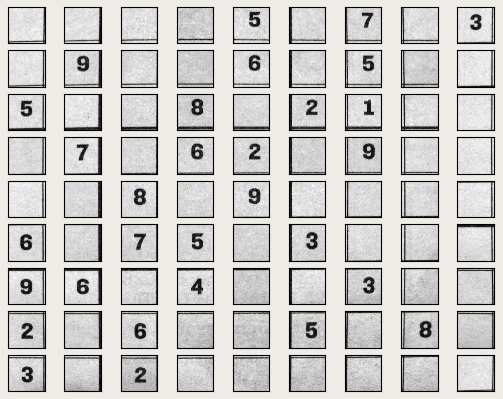
\includegraphics[width=12cm]{Avant_Processing.png}
\end{center}
\vspace{0.5cm} 

\textbf{Avec traitement d'image :}
\begin{center} 
\hspace{15cm}
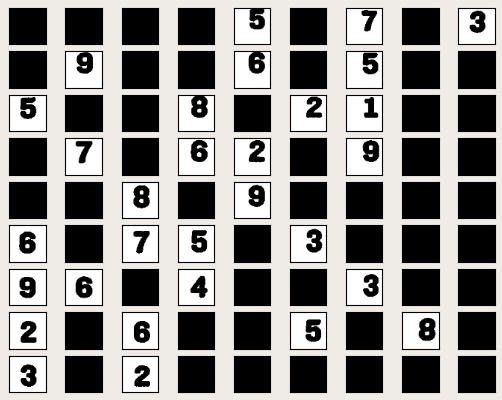
\includegraphics[width=12cm]{Apres_Processing.png}
\end{center}
\vspace{0.5cm} 

Ce qui rend nos cases considérablement plus lisible. Par contre, les cases noires devraient être blanches. Nous n'avons pas compris (même en forcant un valeur soit 0 où 1).

\pagebreak
\section{Noise removal}

Cette partie du filtre consiste à un simple filtre médian qui enlève les petites tâches noires. Il faut tester un peu la force de ce filtre pour que ça filtre, mais pas trop. Voilà une illustration de cette première étape (on remarque que certaine cases sont grises):\\

\textbf{Noise filter:}
\begin{center} 
\hspace{15cm}
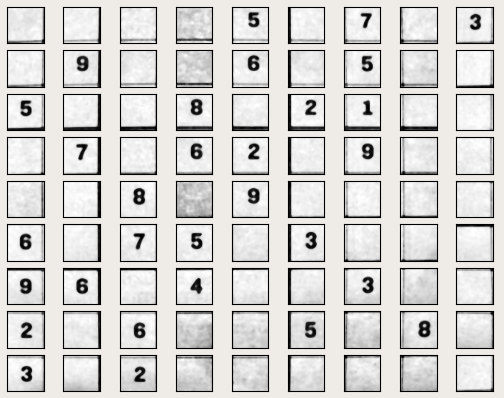
\includegraphics[width=12cm]{Noise_Rem.png}
\end{center}
\vspace{0.5cm} 

maintenant le but est d'essayer de mettre les couleur grise en blanc et les noires en noires. Pour cela nous allons "binariser" l'image avec l'algorithme "OTSU" qui cherche la limite optimale.


\pagebreak
\section{OTSU Thresholding}

Comme dit précédemment, nous allons utiliser un algorithme pour optimiser la "binarisation" d'un image. Voici le résultat de cette opération :\\

\textbf{OTSU threshold:}
\begin{center} 
\hspace{15cm}
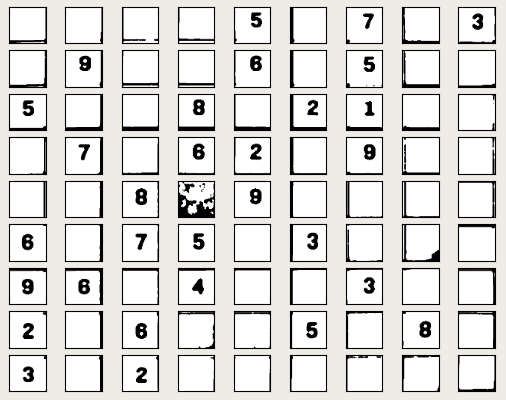
\includegraphics[width=12cm]{OTSU.png}
\end{center}
\vspace{0.5cm} 

On voit quelques impuretés qui trainent encore. On pourrait peut-être passer encore un filtre médian.

\textbf{Second median:}
\begin{center} 
\hspace{15cm}
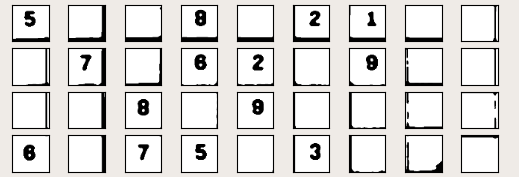
\includegraphics[width=12cm]{median_2.png}
\end{center}
\vspace{0.5cm} 

On voit que cela a bien dégradé nos chiffres, le filtrage est assez bien comme cela, sans ce filtrage supplémentaire. \\
Nos chiffre sont devenu un peut "patates", et c'est pour cela que nous allons les éroder.

\pagebreak
\section{Erosion and border cut}

Le dernière grosse étape consiste à éroder les cases et à couper les bordure (et exécuter un "resize" de l'image bien entendu...).\\
Voici le résultat : \\

\textbf{Erosion and border cut:}
\begin{center} 
\hspace{15cm}
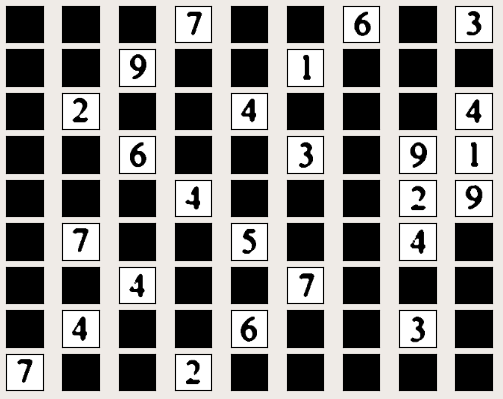
\includegraphics[width=10cm]{Erosion_resize.png}
\end{center}
\vspace{0.1cm} 
Avec cela on obtient un taux de réussite de 100\% sur les meilleures images. Par contre :\\

\textbf{Worst case:}
\begin{center} 
\hspace{15cm}
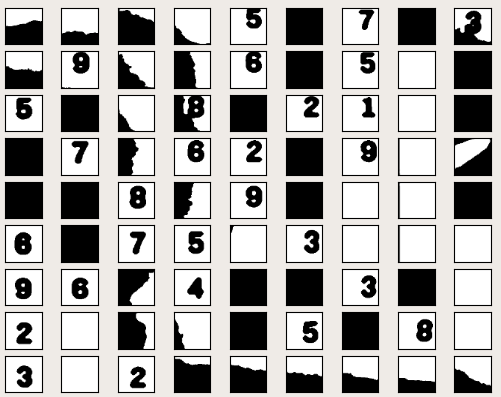
\includegraphics[width=10cm]{Pire_erosion.png}
\end{center}
\vspace{0.1cm} 
On obtient un taux de réussite de 80\%. C'est la solution de traitement qui marche le mieux pour tous. Une bonne image restera toujours un excellent atout pour ce genre de traitement automatisé !

